\documentclass{ctexart}
\usepackage{amsmath,amssymb,amsthm,bm,ulem,graphicx, booktabs}
\usepackage[margin=1 in]{geometry}
\title{数值分析大作业}
\author{数91\and 董浚哲\and 2019011985}
\begin{document}
\maketitle
\newcommand{\R}{\mathbf{R}}
\newcommand{\dd}{\,\mathrm{d}}
\newcommand{\st}{\text{ s.t. }}
\newcommand{\pp}[2]{\frac{\partial #1}{\partial #2}}
\newcommand{\nm}[1]{\left\|#1\right\|}

\subsection*{1.}
设一共有$N$个点$(x_0,y_0),\cdots,(x_{N-1},y_{N-1})$,其中$N=2m$(即要求$N$是偶数)。记$h=\frac{1}{N}$。为计算第一型曲面积分,为曲线取如下的参数化:取$v\in C^\infty([0,1],\R^2) \st v(kh)=(x_k,y_k)\quad\forall k=0,\cdots,n-1$。在这样的参数化下,所需计算的第一型曲线积分为:
\[I=\int_0^1 f(t)\sqrt{(\pp{v}{x})^2+(\pp{v}{y})^2}\dd t=\int_0^1 f(t)|v'(t)|\dd t\]

为给出上述积分的四阶估计,作如下差分:
\begin{itemize}
\item 首先给出等距插值点下的一阶导数的一种四阶估计:
\[f'(x)=\frac{-3f(x-h)-10f(x)+18f(x+h)-6f(x+2h)+f(x+3h)}{12h}+O(h^4)\]
(对于其证明,直接取各项在$x$处的Taylor展开即可。)设这样的差分下得到的$v$的估计为$\tilde{v}$,则$|v'(t)|=|\tilde{v}'(t)|+O(h^4)\Rightarrow I=\int_0^1f(t)|\tilde{v}'(t)|\dd t+O(h^4)$

\item 然后使用复合Simpson求积公式:(众所周知,复合Simpson公式具有4阶精度)
  \[ \int_a^b f(x)\dd x = \frac{2h}{3}[\sum_{k=0}^{m-1}f|\tilde{v}|(x_{2k})+2\sum_{k=1}^mf|\tilde{v}|(x_{2k-1})]\]
    %\sum_{k=1}^n \in\t_{x_{k-1}}^{x_k}f(x)\dd x=\frac{h}{6}\sum_{k=1}^n[f(x_{k-1})+4f(x_{k-\frac 1 2})+f(x_k)]+E_n(f)\]
%其中$E_N(f)=-\frac{1}{2880}(b-a)\frac{1}{n}\sum_{k=1}^N f^{(4)}(\eta_k)$是四阶误差估计。

%为避免选取奇数个插值点出现的问题,对所需计算的积分作如下类型的估计:令$x_k=x_{n+k}\quad k=0,\cdots, n-1$
%\[I=\frac{1}{2}\sum_{k=0}^{n-1}[f(x_{2k})+4f(x_{2k+1})+f(x_{2k+2})]\]
\end{itemize}
%即我们得到如下的四阶估计:取$t_k=t_{k+n}=\frac{k}{n}\quad k=0,\cdots,n-1$,则
%\[I=\frac{1}{2}\sum_{k=0}^{n-1}[f(t_{2k})|\tilde{v}'(t_{2k})|+4f(t_{2k+1})|\tilde{v}'(t_{2k+1})|+f(t_{2k+2})|\tilde{v}'(t_{2k+2})|]\]

\subsection*{2.}

以下算例来自《数学分析》(陈纪修等主编)
\begin{itemize}
\item $\int_{L}|y|\dd s$,其中$L:x^2+y^2=1$。答案:$4$
\item $\int_L |x|^{\frac{1}{3}}\dd s$,其中$L:x^{\frac{2}{3}}+y^{\frac{2}{3}}=1$。答案:$4$
\item $\int_L|x|\dd s$,其中$L:(x^2+y^2)^2=x^2-y^2$。答案:$2\sqrt{2}$
\end{itemize}
计算结果如下:
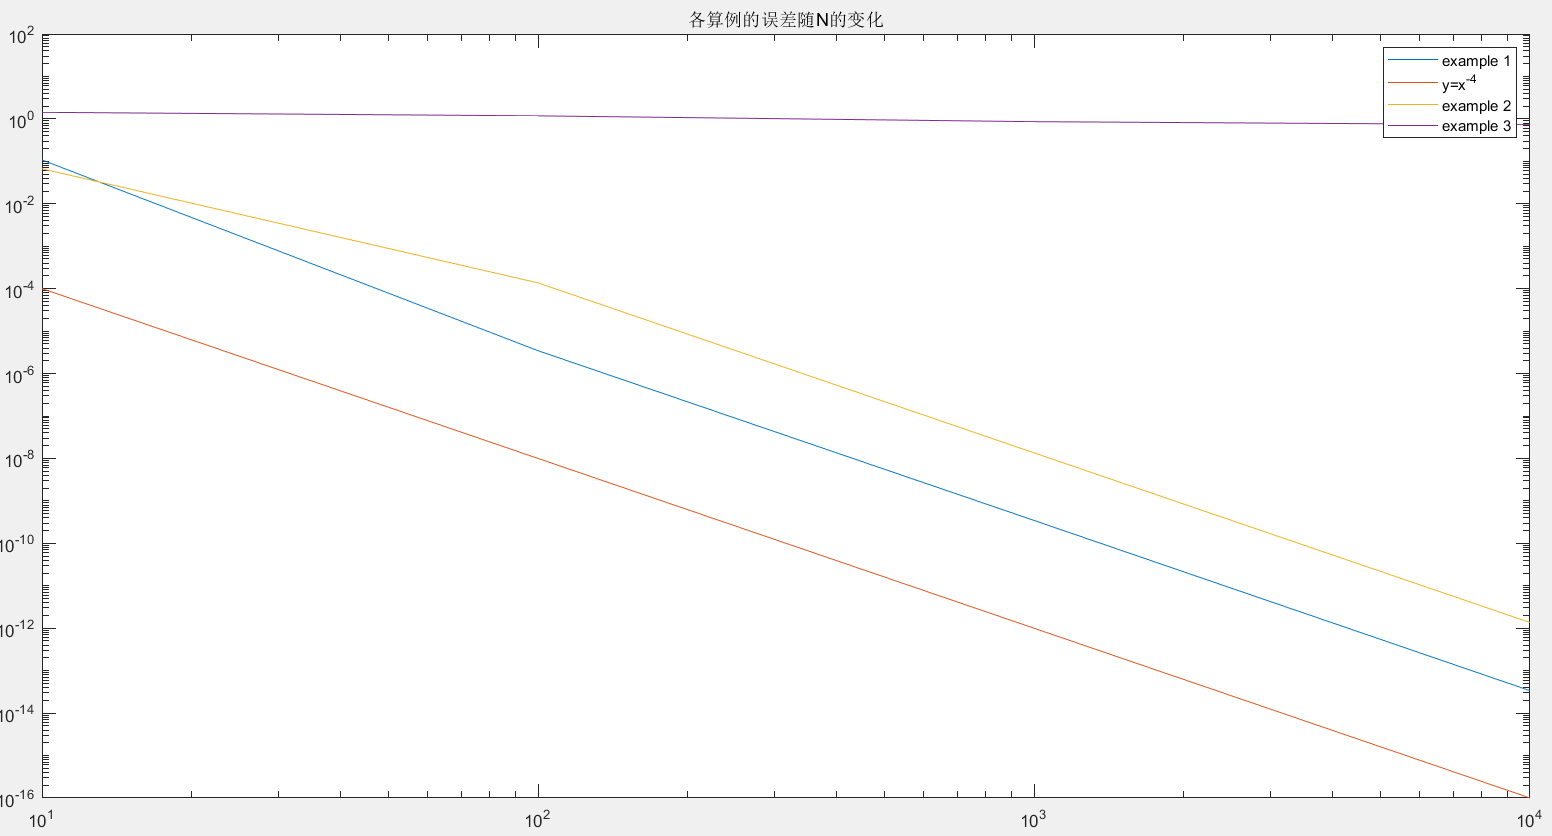
\includegraphics[scale=0.5]{error.bmp}

可见此计算方法可以达到四阶精度,只是稳定性欠佳。









\end{document}